\documentclass[tikz]{standalone}
\usepackage{pgfplots}
\pgfplotsset{compat=1.18}

\begin{document}
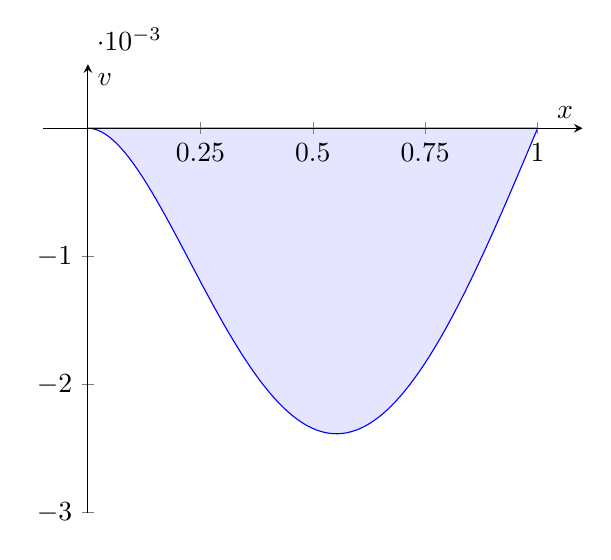
\begin{tikzpicture}
	\begin{axis}[
		axis lines = middle,
		xlabel = $x$,
		ylabel = {$v$},
		xmin=-.1, xmax=1.1,
		ymin=-.003, ymax=0.0005,
		xtick= {0.25, 0.5, 0.75, 1},
		yticklabel style={/pgf/number format/fixed}, % Formato numérico fijo
		set layers, % Activa las capas
		axis on top
		]
		\addplot [
		domain=0:1, 
		samples=100,
		color=blue,
		fill=blue!10,
		]
		{-x^2/30 + x^3/15 - x^4/24 + x^5/120} \closedcycle;
	\end{axis}
\end{tikzpicture}
\end{document}